\section{\texorpdfstring{Klopné obvody}{Klopne obvody}}

% =====================================================================================================================
	\begin{frame}
    \frametitle{RS klopný obvod - Moore}
	
		\begin{minipage}[t][\textheight][t]{0.5\textwidth}
			
			\begin{itemize}
				\item Startem zapni, stopem vypni,
				\item mezi stisky pamatovat stav,
				\item uvažujeme $Y= Q \;\Rightarrow$ Moore,
				\item pozice $x$ řeší prioritu stisku.

			\end{itemize}
			
			\begin{karnaugh-map}[4][2][1][$R$][$S$][$Q$]
				\minterms{2,4,6}
				\indeterminants{3,7}
				\implicant{3}{6}
				\implicantedge{4}{4}{6}{6}
				% ====== vlastní čáry ======

				% A = 1 (druhý řádek)
				\draw[very thick] (-0.15,1) -- (-0.15,0);

				% B = 1 (sloupce 3 a 4)
				\draw[very thick] (2,2.3) -- (4,2.3);

				% C = 1 (sloupce 2 a 3)
				\draw[very thick] (1,2.15) -- (3,2.15);

			\end{karnaugh-map}
			
		\end{minipage}
		\begin{minipage}[t][\textheight][t]{0.45\textwidth}

		\vspace{5mm}
		\begin{center}
			\begin{tabular}{ c c c | c }
				$Q$ & $S$ & $R$ & Q \\
				\hline
				0 & 0 & 0 & 0 \\
				0 & 0 & 1 & 0 \\
				0 & 1 & 0 & 1 \\
				0 & 1 & 1 & $x$ \\
				1 & 0 & 0 & 1 \\
				1 & 0 & 1 & 0 \\
				1 & 1 & 0 & 1 \\
				1 & 1 & 1 & $x$ \\
			\end{tabular}
			
			\vspace{4mm}
			$Q= \textcolor{red}{S}+\textcolor{green}{\bar{R}Q}$
		\end{center}

		\end{minipage}
	
	\end{frame}
	
% =====================================================================================================================
	\begin{frame}
    \frametitle{RS klopný obvod - zapojení}
		\small
		\begin{enumerate}
			\item Úprava na NAND - De Morganovy zákony:
			\begin{align*}
				Q=& S+\bar{R}Q = \bar{\bar{Q}} = \overline{\overline{S+\bar{R}Q}} = \\
				 =& \overline{\bar{S} \cdot \overline{\bar{R}Q}}
			\end{align*}
			
			\item Zapojení:
				
				\begin{center}
					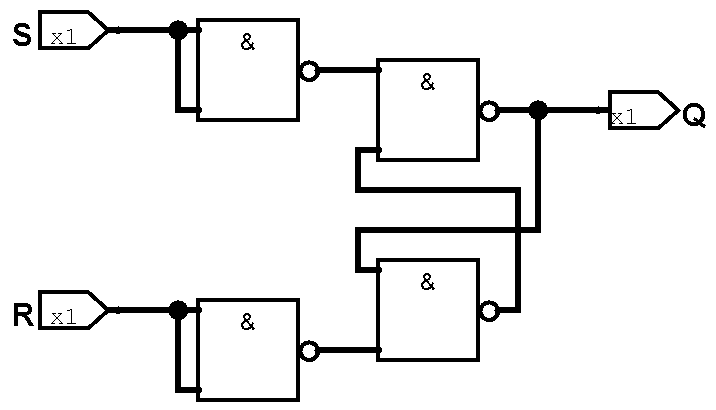
\includegraphics[width=0.5\textwidth]{fig/RS_KO.png}
				\end{center}
		\end{enumerate}
	
	\end{frame}
	
% =====================================================================================================================
	\begin{frame}
    \frametitle{RST klopný obvod - zapojení}
		\small
		\begin{enumerate}
			\item Zavádíme navíc signál T (Toggle) pro povolení vstupů:
			\begin{align*}
				Q=& TS+\overline{TR}Q = \bar{\bar{Q}} = \overline{\overline{TS+\overline{TR}Q}} = \\
				 =& \overline{\overline{TS} \cdot \overline{\overline{TR}Q}}
			\end{align*}
			\item Zapojení:
				
				\begin{center}
					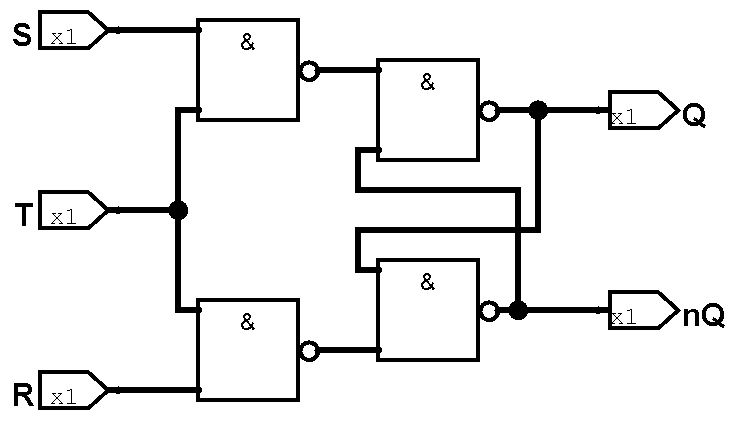
\includegraphics[width=0.5\textwidth]{fig/RST_KO.png}
				\end{center}
		\end{enumerate}
	
	\end{frame}
  
% =====================================================================================================================
	\begin{frame}
    \frametitle{D klopný obvod - zapojení}
		\small
		\begin{itemize}
			\item RST KO zapojené do kaskády:
				
				\begin{center}
					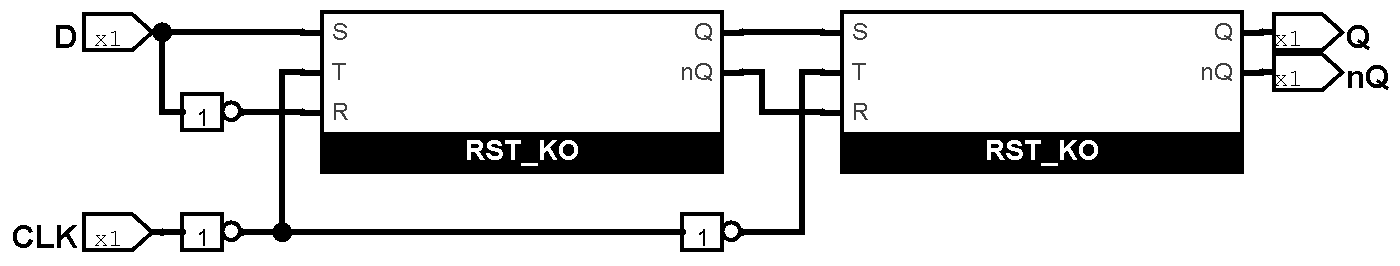
\includegraphics[width=0.8\textwidth]{fig/D_KO.png}
				\end{center}
        
      \item Vstup D (Data) slouží k nastavení budoucí hodnoty,
      \item stav je změněn jen při příchodu náběžné hrany na vstupu CLK (Clock),
      \item reakci na sestupnou hranu lze získat odstraněním první negace vstupu CLK.
		\end{itemize}
	
	\end{frame}
  
% =====================================================================================================================
	\begin{frame}
    \frametitle{D klopný obvod - hradlo 74HC74}
		\small
		\begin{itemize}
			\item RST KO zapojené do kaskády:
				
				\begin{center}
					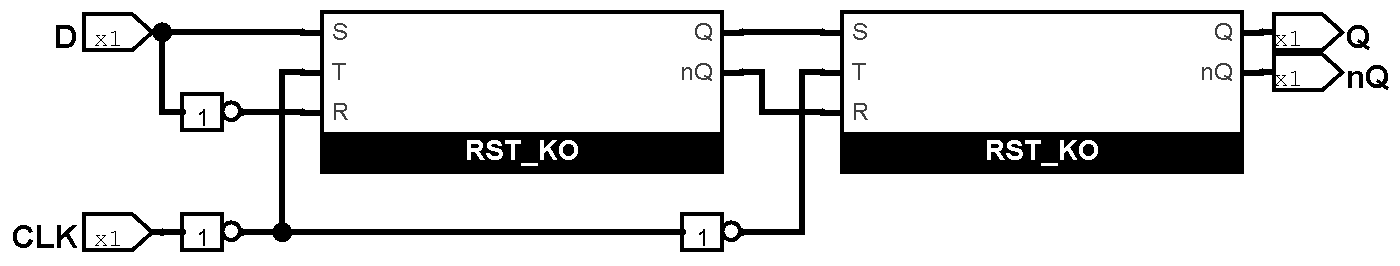
\includegraphics[width=0.8\textwidth]{fig/D_KO.png}
				\end{center}
        
      \item Vstup D (Data) slouží k nastavení budoucí hodnoty,
      \item stav je změněn jen při příchodu náběžné hrany na vstupu CLK (Clock),
      \item reakci na sestupnou hranu lze získat odstraněním první negace vstupu CLK.
		\end{itemize}
	
	\end{frame}